\pgfplotsset{compat=1.18}
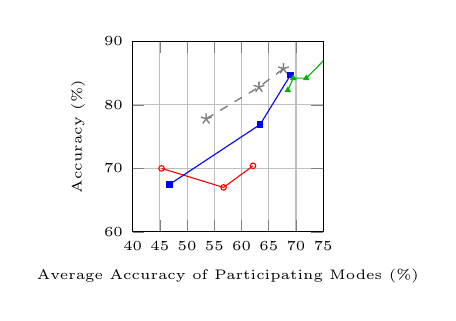
\begin{tikzpicture}
\begin{axis}[
    width=0.33\textwidth, height=0.33\textwidth,
    xlabel={Average Accuracy of Participating Modes (\%)},
    ylabel={\tiny{Accuracy (\%)}},
    tick label style={font=\tiny},
    label style={font=\tiny},
    legend style={at={(0.5,-0.25)}, anchor=north, legend columns=2, font=\tiny},
    grid=both,
    xmin=40, xmax=75,
    ymin=60, ymax=90,
    xtick={40, 45, 50, 55, 60, 65, 70, 75},
    ytick={60, 70, 80, 90}
]


% Code ×3 Vote
\addplot[color=red, mark=o, mark size=1pt] coordinates {
    (45.3, 70.0)
    (56.7, 67.00)
    (62.1, 70.4)
};
% \addlegendentry{Code $\times$3 Vote};

% Truth Table ×3 Vote
\addplot[color=blue, mark=square*, mark size=1pt] coordinates {
    (46.8, 67.5)
    (63.4, 76.9)
    (69.0, 84.7)
    (69.0, 84.7)
};
% \addlegendentry{Truth Table $\times$3 Vote};

% NL-CoT ×3 Vote
\addplot[color=green!70!black, mark=triangle*, mark size=1pt] coordinates {
    (68.5, 82.3)
    (69.5, 84.2)
    (71.9, 84.2)
    (75.9, 87.7)
};
% % \addlegendentry{NL-CoT $\times$3 Vote};


% Mixture Upper Bound
\addplot[color=gray, dashed, mark=star] coordinates {
    (53.5, 77.8)
    (63.2, 82.8)
    (67.7, 85.7)
};


% \addplot[color=blue, mark=square*, mark size=1pt] coordinates {
%     (45.3, 70.0)
%     (46.8, 67.5)
%     (56.7, 67.00)
%     (62.1, 70.4)
%     (63.4, 76.9)
%     (68.5, 82.3)
%     (69.0, 84.7)
%     (69.5, 84.2)
%     (71.9, 84.2)
%     (75, 87)
% };
% \addlegendentry{Truth Table $\times$3 Vote};


% Mixture Upper Bound
\addplot[color=gray, dashed, mark=star] coordinates {
    (53.5, 77.8)
    (63.2, 82.8)
    (67.7, 85.7)
};

% \addlegendentry{Mixture Upper Bound};

\end{axis}
\end{tikzpicture}